\section{Auswertung}
\label{sec:Auswertung}

% \begin{figure}
%   \centering
%   \includegraphics{plots/plot.pdf}
%   \caption{Plot.}
%   \label{fig:plot}
% \end{figure}



% \begin{table}
%    % Notation :  {% nicht entfernen ist sehr wichtig sonst Fehler !!
% \parbox{0.48\textwidth}{% %Ermöglicht zwei Tabellen neben einander
%   \centering
%   \sisetup{round-mode = places , round-precision = 0,scientific-notation=fixed, fixed-exponent = 0}
%          %rundet Werte aus Stelle, Stelle = ,  macht einen bestimmten festen exponenten
%   \resizebox{\textwidth}{!}{%  % skaliert zu große Tabellen
%   \begin{tabular}{S@{${}\pm{}$} S} % fügt plus minus Fehler Schreibweise hinzu
%     \toprule
%      $\text{e}_b / \si{\milli\meter}$ &
%      $\text{d}_b /\si{\milli\meter} $ & $\text{f}_b / \si{\milli\meter} $\\
%     \midrule
%     \bottomrule
%   \end{tabular}
%   % }
%   \caption{Tabellenunterschrift}
%   \label{tab:tab}
% }
% % \end{table}
% % \begin{table}
% \parbox{0.48\textwidth}{%
%   \centering
%   \sisetup{round-mode = places , round-precision = 0,scientific-notation=fixed, fixed-exponent = 0}
%   % \resizebox{\textwidth}{!}{%
%   \begin{tabular}{S@{${}\pm{}$} S}
%     \toprule
%      $\text{e}_b / \si{\milli\meter}$ &
%      $\text{d}_b /\si{\milli\meter} $ & $\text{f}_b / \si{\milli\meter} $\\
%     \midrule
%     \bottomrule
%   \end{tabular}
%   % }
%   \caption{Tabellenunterschrift}
%   \label{tab:tab}
% }
% \end{table}
Im Folgenden werden die Fits, Plots und Fehlerrechnungen mit den Paketen Numpy \cite{numpy}, Uncertainties \cite{uncertainties},
Matplotlib \cite{matplotlib} und Scipy \cite{scipy} in der Programmierumgebung Pyhton 3.6.0 erstellt bzw. durchgeführt.
\subsection{Volumenbestimmung}
Um das Saugvermögen der Pumpen zu bestimmen muss zuerst das Volumen der verwendeten Apparatur bestimmt werden. Dabei ist
darauf zu achten, dass das Gesamtvolumen des Aufbaues für die beiden Pumpen unterschiedlich groß ist.\\
Hierzu werden für die meisten Bauteile die Angaben aus \cite{Anleitung} verwendet.\\
Ein weiteres verwendetes Bauteil wurde vermessen und wird, da es gut als Zylinder genähert werden kann, mit
\begin{equation}
  V_{\text{Zylinder}}=\pi r^2 h, \qquad \sigma_{V}=\sqrt{4 \pi^{2} h^{2} r^{2} \sigma_{r}^{2}  + \pi^{2} r^{4} \sigma_{h}^{2} }
\label{eq:VolumenZylinder}
\end{equation}
bestimmt. In \ref{eq:VolumenZylinder} wurde der Fehler des bestimmten Volumens mittels Gaußscher Fehlerfortpflanzung gleich mitbedacht.\\
Allgemein wird diese für eine Funktion $f$ mit $M$ Variablen $x_i$ über
\begin{equation}
  \label{eq:GaussFehler}
  \sigma_f= \sqrt{ \sum_i^M \left(\frac{\partial f}{\partial x_i} \sigma_{x_i}\right)^2}.
\end{equation}
berechnet.\\
Für das zu berechnende Verbindungsstück wurden für den Innendurchmesser $d=(12,00 \pm 0,05)$ mm und für die Läge $L=(61\pm 1)$ mm vermessen.
Damit ergibt sich mit \ref{eq:VolumenZylinder} für das Volumen $V=(6900 \pm 130)\,\text{mm}^3 = (0,0069 \pm 0,0001)$\,l.
Da bei den unterschiedlichen Versuchsteilen unteranderem die Ventile mal geöffnet und mal geschlossen sind wird eine weitere Unterteilung
für die Unterschiedlichen Messungen gemacht. Die Kugelventile befinden sich in Position 3,5 und vor der Turbopumpe in Bild \ref{fig:Aufbau}.
Das Klappenventil ist über dem Bauteil 6 zu finden und das Handventil schließt die Verbindung der Drehschieberpumpe an den Schlauch 9 und ist nicht mehr
auf dem Bild zu sehen.\\
In den Tabellen \ref{tab:Volumen_ET},\ref{tab:Volumen_LT},\ref{tab:Volumen_ED} und \ref{tab:Volumen_LD} sind die verwendeten Bauteile
 und ihr jeweiliges Volumen aufgetragen.
Die Einzelvolumina werden aufaddiert und der Fehler mit Formel \ref{eq:GaussFehler} bestimmt.

\begin{table}[H]
\centering
\caption{Werte zur Bestimmung des Gesamtvolumen der Apparatur bei der Evakuierungsmessung der Turbomolekularpumpe.}
\label{tab:Volumen_ET}
\begin{tabular}{c|c}
Bauteil & Voumen $V$ in l\\
\hline
Tank &$9,5 \pm 0,8$\\
langer Schlauch &$0,8 \pm 0,1$\\
kurzer Schlauch &$0,087 \pm 0,011$\\
T-Stück klein&$0,013 \pm 0,002$\\
T-Stück groß &$0,25 \pm 0,01$\\
Kreuzstück klein&$0,016 \pm 0,002$\\
Kreuzstück groß&$0,177 \pm 0,09$\\
Verbindungsstück&$0,0069 \pm 0,0001$\\
Querschnittsverengung&$0,067 \pm 0,004$\\
1 offenes Kugelventil&$0,015 \pm 0,002$\\
2 geschlossene Kugelventile&$ 2 \cdot(0,005 \pm 0,001)$\\
1 offenes Klappenventil&$0,044 \pm 0,004$\\
1 offenes Handventil&$0,025\pm0,005$\\
\hline
Gesamtvolumen&$11,0 \pm 0,8$\\
\end{tabular}
\end{table}

\begin{table}[H]
\centering
\caption{Werte zur Bestimmung des Gesamtvolumen der Apparatur bei der Leckratenmessung der Turbomolekularpumpe.}
\label{tab:Volumen_LT}
\begin{tabular}{c|c}
Bauteil & Voumen $V$ in l\\
\hline
Tank &$9,5 \pm 0,8$\\
T-Stück groß &$0,25 \pm 0,01$\\
Kreuzstück groß&$0,177 \pm 0,09$\\
Querschnittsverengung&$0,067 \pm 0,004$\\
2 geschlossene Kugelventile&$ 2 \cdot(0,005 \pm 0,001)$\\
1 offenes Klappenventil&$0,044 \pm 0,004$\\
\hline
Gesamtvolumen&$10,0\pm0,8$\\
\end{tabular}
\end{table}

\begin{table}[H]
\centering
\caption{Werte zur Bestimmung des Gesamtvolumen der Apparatur bei der Evakuierungsmessung der Drehschieberpumpe.}
\label{tab:Volumen_ED}
\begin{tabular}{c|c}
Bauteil & Voumen $V$ in l\\
\hline
Tank &$9,5 \pm 0,8$\\
langer Schlauch &$0,8 \pm 0,1$\\
kurzer Schlauch &$0,087 \pm 0,011$\\
T-Stück klein&$0,013 \pm 0,002$\\
T-Stück groß &$0,25 \pm 0,01$\\
Kreuzstück klein&$0,016 \pm 0,002$\\
Kreuzstück groß&$0,177 \pm 0,09$\\
Verbindungsstück&$0,0069 \pm 0,0001$\\
Querschnittsverengung&$0,067 \pm 0,004$\\
1 offenes Kugelventil&$0,015 \pm 0,002$\\
2 geschlossene Kugelventile&$ 2 \cdot(0,005 \pm 0,001)$\\
1 geschlossenes Klappenventil&$\frac{1}{2}\cdot(0,044 \pm 0,004)$\\
1 offenes Handventil&$0,025 \pm 0,005$\\
\hline
Gesamtvolumen&$11,0 \pm 0,8$\\
\end{tabular}
\end{table}

\begin{table}[H]
\centering
\caption{Werte zur Bestimmung des Gesamtvolumen der Apparatur bei der Leckratenmessung der Drehschieberpumpe.}
\label{tab:Volumen_LD}
\begin{tabular}{c|c}
Bauteil & Voumen $V$ in l\\
\hline
Tank &$9,5 \pm 0,8$\\
langer Schlauch &$0,8 \pm 0,1$\\
kurzer Schlauch &$0,087 \pm 0,011$\\
T-Stück klein&$0,013 \pm 0,002$\\
T-Stück groß &$0,25 \pm 0,01$\\
Kreuzstück klein&$0,016 \pm 0,002$\\
Kreuzstück groß&$0,177 \pm 0,09$\\
Verbindungsstück&$0,0069 \pm 0,0001$\\
Querschnittsverengung&$0,067 \pm 0,004$\\
2 offenes Kugelventil&$2\cdot(0,015 \pm 0,002)$\\
1 geschlossene Kugelventile&$ 0,005 \pm 0,001$\\
1 geschlossenes Klappenventil&$\frac{1}{2}\cdot(0,044 \pm 0,004)$\\
1 geschlossenes Handventil&$\frac{1}{2}\cdot(0,025 \pm 0,005)$\\
\hline
Gesamtvolumen&$11,0 \pm 0,8$\\
\end{tabular}
\end{table}
\subsection{Drehschieberpumpe}
Der Vollständigkeit halber muss erwähnt werden, dass die im folgenden aufgeführten Zeitmessungen
über eine Smartphone Stopp-Uhr aufgenommen worden. Deswegen ist zu beachten,
dass alle gemessenen Werte einem systematischen Fehler unterliegen, der hauptsächlich durch die Reaktionsschnelle des Messenden gegeben ist.
Die Reaktionszeit eines Menschen auf einen visuellen Reiz beträgt ca. 180 ms \cite{Reaktion}.
Da alle Messungen diesem Fehler unterliegen, wird er im folgenden vernachlässigt.
\subsubsection{Evakuierungsmessung}
Die in Tabelle \ref{tab:EvakuierungskurveDrehschieber} aufgetragenen Drücke $p$ haben durch die Messungenauigkeit der
der logarithmischen Anzeige des analogen Piranimessgerät einen Fehler von $\pm 20$\%.
Die für die Auswertung der Evakuierungskurve benötigten Mittelwerte der gemessenen Zeiten $t$ werden mit
\begin{equation}
  \label{eq:mittelwert}
  \bar{x}=\frac{1}{N}\sum_i^N x_i
\end{equation}
berechnet. Die zugehörige Standardabweichung des Mittelwertes lautet:
\begin{equation}
  \label{eq:standartabweichung}
  \sigma_{\bar{x}}=\sqrt{ \frac{1}{N(N-1)} \sum_i^N (x_i-\bar{x})^2}.
\end{equation}
Da für die Funktion $f=ln\left(\frac{p(t)-p_\symup{E}}{p_0-p_\symup{E}}\right)$ fehlerbehaftete Werte verwendet werden,
muss der sich ergebende Fehler mit Formel \ref{eq:GaussFehler} zu
\begin{equation}
  \label{eq:FehlerLnDruck}
  \sigma_{ln(p)}=\sqrt{\frac{\sigma_{p}^{2}}{\left(p - p_\symup{E}\right)^{2}} + \frac{\sigma_{p_{0}}^{2}}{\left(p_{0} - p_\symup{E}\right)^{2}} + \frac{\sigma_{p_\symup{E}}^{2}
   \left(p_{0} - p_\symup{E}\right)^{2}}{\left(p - p_\symup{E}\right)^{2}} \left(\frac{p - p_\symup{E}}{\left(p_{0} - p_\symup{E}\right)^{2}} - \frac{1}{p_{0} - p_\symup{E}}\right)^{2}}.
\end{equation}
bestimmt werden.

\begin{table}[H]
\centering
\caption{Messwerte zur Bestimmung der Evakuierungskurve der Drehschieberpumpe.}
\label{tab:EvakuierungskurveDrehschieber}
\begin{tabular}{c|c|c|c|c|c|c|c}
  \toprule
$p$/\,mbar & $ln\left(\frac{p(t)-p_\symup{E}}{p_0-p_\symup{E}}\right)$ & $t_1$/\,s & $t_2$/\,s & $t_3$/\,s & $t_4$/\,s & $t_5$/\,s & $t_\symup{m}$/\,s\\
\midrule
$100   \pm \, 20$ & $-2,3 \pm \, 0,3$ &9,57 & 11,689 & 12,21 & 15,349 & 13,910 & $12,546 \pm \, 0,98$\\
$40    \pm \, 8$ & $-3,2 \pm \, 0,3   $&22,160 & 23,579 & 23,640 & 28,500 & 23,910 &$ 24,3579 \pm \, 1,079$\\
$20    \pm \, 4$ & $-4,0 \pm \, 0,3 $& 27,839 & 30,940 & 31,250 & 36,100 & 31,059 &$ 31,4379 \pm \, 1,324$\\
$10    \pm \, 2$ & $-4,6 \pm \, 0,3 $ & 35,270 & 38,079 & 38,219 & 43,109 & 38,520 &$ 38,6400 \pm \, 1,261$\\
$4     \pm \, 0,800 $&$ -5,5 \pm \, 0,3 $ & 44,03 & 47,020 & 47,049 & 51,729 & 47,179 &$ 47,402 \pm \, 1,233$\\
$2     \pm \, 0,400 $&$ -6,2 \pm \, 0,3 $& 50,45 & 53,299 & 53,539 & 58,659 & 54,229 &$ 54,036 \pm \, 1,324$\\
$1     \pm \, 0,200 $&$ -6,9 \pm \, 0,3 $ & 57,57 & 60,859 & 60,740 & 65,819 & 60,859 &$ 61,170 \pm \, 1,322$\\
$0,4   \pm \, 0,08 $& $ -7,9 \pm \, 0,3$& 69,9399 & 73,7199 & 73,6899 & 79,6800 & 73,7199 &$ 74,1500 \pm \, 1,563$\\
$0,2   \pm \, 0,04$&$-8,6 \pm \, 0,3  $& 82,4800 & 85,8900 & 86,0100 & 91,0600 & 85,9500 &$ 86,2779 \pm \, 1,371$\\
$0,1   \pm \, 0,02$ &$ -9,3 \pm \, 0,3 $& 93,1800 & 96,5999 & 96,7900 & 102,09 & 100,519 &$ 97,8359 \pm \, 1,574$\\
$0,004 \pm \, 0,0008$ &$ -10,5 \pm \, 0,4$  & 132,099 & 134,550 & 133,689 & 140,879 & 133,879 &$ 135,020 \pm \, 1,519$\\
$0,002 \pm \, 0,0004$ & $ -11,7 \pm \, 0,6$  & 199,500 & 204,340 & 202,080 & 219,139 & 202,060 &$ 205,424 \pm \, 3,513$\\
\bottomrule
\end{tabular}
\end{table}
Die in Tabelle \ref{tab:EvakuierungskurveDrehschieber} aufgetragenen Messwerte für den Druck sind in Abbildung \ref{fig:EvaDrehExp} in
dargestellt.
\begin{figure}[H]
  \centering
  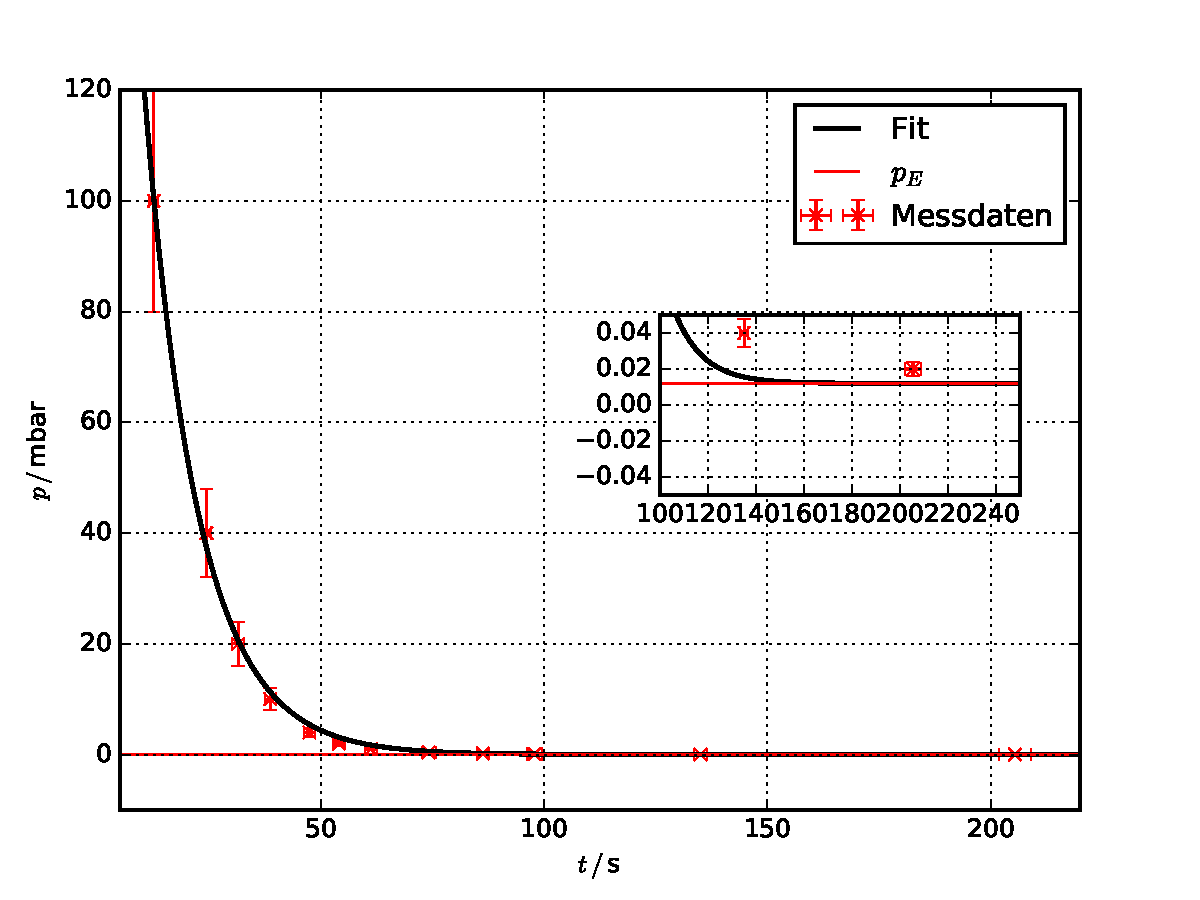
\includegraphics[width=0.7\textwidth]{plots/EvakuierungDrehExp.pdf}
  \caption{Plot der in Tabelle \ref{tab:EvakuierungskurveDrehschieber} aufgelisteten Messwerte mit exponentiellem Fit. Zusätzlich ist eine Vergrößerung
  des Bereichs 100\,s$\leq t\leq$240\,s dargestellt.}
  \label{fig:EvaDrehExp}
\end{figure}
Der in Abbildung \ref{fig:EvaDrehExp} verwendetet Fit folgt der Funktion
\begin{equation}
   f(x)=a\cdot\exp(b\cdot (-x))+c
  \label{eq:Drehexpfit}
\end{equation}
dabei wurde für den Parameter $c$ der Enddruck $p_\symup{E}=0,012$\,mbar angegeben. Die anderen Parameter wurden zu
\begin{align}
  a&= (287 \pm 8)\,\,\symup{mbar}\\
  b&= (0,084 \pm 0,002)\,\frac{1}{\symup{s}}
\end{align}
bestimmt.
Aus dem Parameter $b$ lässt sich nun ein gemitteltes Saugvermögen $S_\symup{g}$ berechnen.
Aus Gleichung \ref{eq:pt} folgt $b=\frac{S}{V}$. Mit einem Volumen von $V=(11,0 \pm 0,8)$\,l und ergibt sich:
\begin{equation}
  S_\symup{g}= b \cdot V =(0,084 \m 0,002)\,\frac{1}{\symup{s}} \cdot (11,0 \pm 0,8)\,\symup{l} =(0,92 \pm 0,07)\,\frac{\symup{l}}{\symup{s}}
  \label{eq:Saugvermögen}
\end{equation}
Da das Saugvermögen im allgemeinen nicht unabhängig vom Druck ist, anders als in der Herleitung der Gleichung \ref{eq:pt} angenommen,
wird eine von Druckbereichen abhängige Untersuchung vorgenommen.
In Abbildung \ref{fig:EvaDrehLin} sind die logarithmirten Werte gegen die Zeit aufgetragen.
\begin{figure}[H]
  \centering
  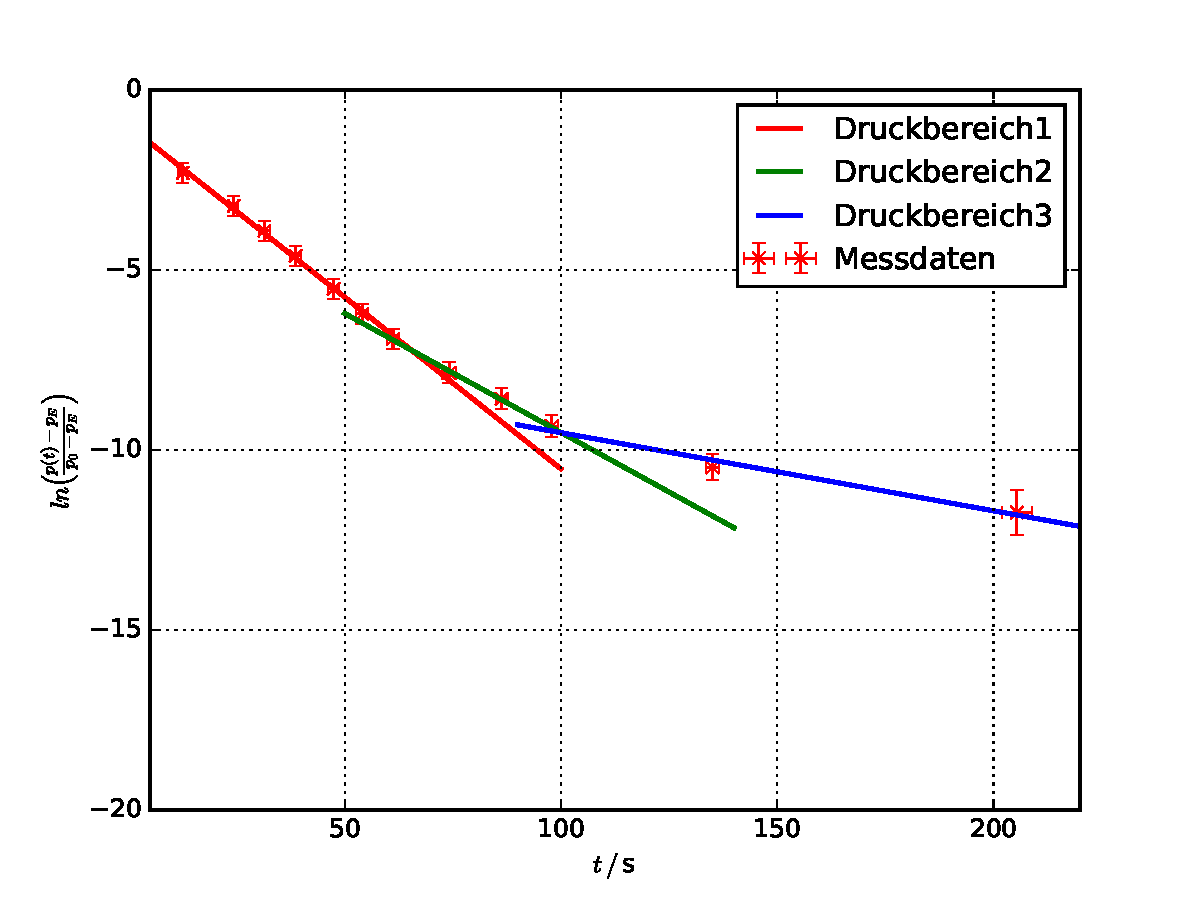
\includegraphics[width=0.7\textwidth]{plots/EvakuierungDrehlin.pdf}
  \caption{Plot der in Tabelle \ref{tab:EvakuierungskurveDrehschieber} aufgelisteten Messwerte mit linearen Fits der einzelnen Teilbereichen.}
  \label{fig:EvaDrehLin}
\end{figure}
Wie in der Abbildung \ref{fig:EvaDrehLin} zu erkennen, gibt es drei lineare Bereiche. %,
In diesen Bereichen werden an die Messdaten jeweils eine Gerade der Form
\begin{equation}
  \label{eq:Geradengleichung}
  g(x)=mx+b
\end{equation}
gefittet.
Mit Hilfe von Regressionsberechnungen werden die Parameter der einzelnen Geraden bestimmt.
Um das Saugvermögen $S=-a\cdot V$ zu bestimmen wird jetzt die Steigung $a$ verwendet:
\begin{align}
  \label{eq: regression_dreh_druck_1}
  \begin{aligned}
  \text{Druckbereich 1} \quad  & 2\,\symup{mbar}\leq p \leq 100\,\symup{mbar} \\
  m&= -0,095 \pm 0,003 \frac{1}{\symup{s}}\\
  b&= -1,0 \pm 0,1\\
  S_1&= (1,05 \pm 0,08)\,\frac{\symup{l}}{\symup{s}}
\end{aligned}
\end{align}
\begin{align}
  \label{eq: regression_dreh_druck_2}
  \begin{aligned}
  \text{Druckbereich 2} \quad  & 0,2\,\symup{mbar}\leq p \leq 1\,\symup{mbar} \\
  m&= -0.066 \pm 0,004 \frac{1}{\symup{s}}\\
  b&= -2,9 \pm 0,3\\
  S_2&= (0,73 \pm 0,07)\,\frac{\symup{l}}{\symup{s}}
\end{aligned}
\end{align}
\begin{align}
  \label{eq: regression_dreh_druck_3}
  \begin{aligned}
  \text{Druckbereich 2} \quad  & 0,02\,\symup{mbar}\leq p \leq 0,1\,\symup{mbar} \\
  m&= (-0,022 \pm 0,003) \frac{1}{\symup{s}}\\
  b&= -7,3 \pm 0,5\\
  S_3&=(0,24 \pm 0,04)\,\frac{\symup{l}}{\symup{s}}
\end{aligned}
\end{align}
\subsubsection{Leckratenmessung}
\begin{table}[H]
\centering
\caption{Messwerte der Leckratenmessung der Drehschieberpumpe mit Gleichgewichtsdruck $p_\symup{g}=0,1$\, mbar.}
\label{tab:leck_Dreh1}
\begin{tabular}{c|c|c|c|c}
  \toprule
$p$/\,mbar & $t_1$/\,s & $t_2$/\,s & $t_3$/\,s & $t_\symup{m}$/\,s\\
\midrule
$(0,2 \pm 0,04)$&   10,97&  13,59&  14,97& $(13 \pm 1)$\\
$(0,3 \pm 0,06)$&    27,9&  29,63&  29,97& $(29,2 \pm 0,6) $\\
$(0,4 \pm 0,08)$&   49,15&  49,91&  49,45& $(49,5 \pm 0,2) $\\
$(0,5 \pm 0,1)$&   63,49&  65,36&  65,27& $(64,7 \pm 0,6) $\\
$(0,6 \pm 0,12)$&   80,91&  83,10&  84,01& $(82,7 \pm 0,9) $\\
$(0,7 \pm 0,14)$&  104,43& 105,74& 105,24& $(105,1 \pm 0,4) $\\
$(0,8 \pm 0,16)$&  120,23& 124,02& 123,86& $(123 \pm 1) $\\
\bottomrule
\end{tabular}
\end{table}
\begin{table}[H]
\centering
\caption{Messwerte der Leckratenmessung der Drehschieberpumpe mit Gleichgewichtsdruck $p_\symup{g}=0,4$\, mbar.}
\label{tab:leck_Dreh2}
\begin{tabular}{c|c|c|c|c}
  \toprule
$p$/\,mbar & $t_1$/\,s & $t_2$/\,s & $t_3$/\,s & $t_\symup{m}$/\,s\\
\midrule
$(1 \pm 0,2)   $&20,18&  20,39&  19,48&$(20,0 \pm 0,3) $\\
$(1,5 \pm 0,3) $&31,77&  33,25&  32,43&$(32,5 \pm 0,4) $\\
$(2 \pm 0,4)   $&50,87&  52,66&  51,41&$(51,6 \pm 0,5) $\\
$(2,5 \pm 0,5) $&64,74&  65,97&  66,19&$(65,6 \pm 0,5) $\\
$(3 \pm 0,6)   $&80,20&  80,11&  79,38&$(79,9 \pm 0,3) $\\
$(3,5 \pm 0,7) $&99,70&  99,94&  99,94&$(99,86 \pm 0,08) $\\
$(4 \pm 0,8)   $&127,1& 124,27& 127,43&$(126 \pm 1)$\\
\bottomrule
\end{tabular}
\end{table}
\begin{table}[H]
\centering
\caption{Messwerte der Leckratenmessung der Drehschieberpumpe mit Gleichgewichtsdruck $p_\symup{g}=0,4$\, mbar.}
\label{tab:leck_Dreh3}
\begin{tabular}{c|c|c|c|c}
  \toprule
$p$/\,mbar & $t_1$/\,s & $t_2$/\,s & $t_3$/\,s & $t_\symup{m}$/\,s\\
\midrule
$(2 \pm 0,)$&  17,83&  18,23&   17,7&$(17,9 \pm 0,2)$\\
$(3 \pm 0,)$&  29,13&  29,56&  28,82&$(29,2 \pm 0,2)$\\
$(4 \pm 0,)$&  51,04&  48,94&  48,42&$(49,5 \pm 0,8)$\\
$(5 \pm 0,)$&  63,62&  63,57&  62,97&$(63,4 \pm 0,2)$\\
$(6 \pm 0,)$&  79,68&  81,27&  79,22&$(80,1 \pm 0,6)$\\
$(7 \pm 0,)$& 106,97& 105,83& 107,01&$(106,6 \pm 0,4)$\\
$(8 \pm 0,)$& 123,16& 127,22& 123,07&$(124 \pm 1)$\\
\bottomrule
\end{tabular}
\end{table}
\begin{table}[H]
\centering
\caption{Messwerte der Leckratenmessung der Drehschieberpumpe mit Gleichgewichtsdruck $p_\symup{g}=1$\, mbar.}
\label{tab:leck_Dreh4}
\begin{tabular}{c|c|c|c|c}
  \toprule
$p$/\,mbar & $t_1$/\,s & $t_2$/\,s & $t_3$/\,s & $t_\symup{m}$/\,s\\
\midrule
$(2 \pm 0,4)$&   10,33&  10,45&   9,99& $(10,3 \pm 0,1)$\\
$(3 \pm 0,6)$&   19,98&  18,53&  19,65& $(19,4 \pm 0,4)$\\
$(4 \pm 0,8)$&   34,64&  33,15&  30,51& $(33 \pm 1)$ \\
$(5 \pm 1)$&   44,01&  44,24&  42,24& $(43 \pm 1)$  \\
$(6 \pm 1,2)$&   57,81&  55,82&  54,51& $(56 \pm 1)$ \\
$(7 \pm 1,4)$&   75,91&  75,57&  74,43& $(75,3 \pm 0,4)$\\
$(8 \pm 1,6)$&   89,78&  86,33&  87,44& $(88 \pm 1)$ \\
$(9 \pm 1,8)$&  103,05& 104,70&  95,94& $(101 \pm 3)$ \\
$(10 \pm 2)$& 126,90& 122,17& 133,25& $(127 \pm 3)$ \\
\bottomrule
\end{tabular}
\end{table}
In den Graphiken \ref{fig:leck_dreh_groß1} und \ref{fig:leck_dreh_groß2} sind die Messwerte der vier Leckratenmessungen graphisch aufgetragen.
Es wurden mittels linearer Regression Ausgleichsgeraden der Form \ref{eq:Geradengleichung} bestimmt.
\begin{figure}
    \centering
    \begin{subfigure}{0.45\textwidth}
        \centering
        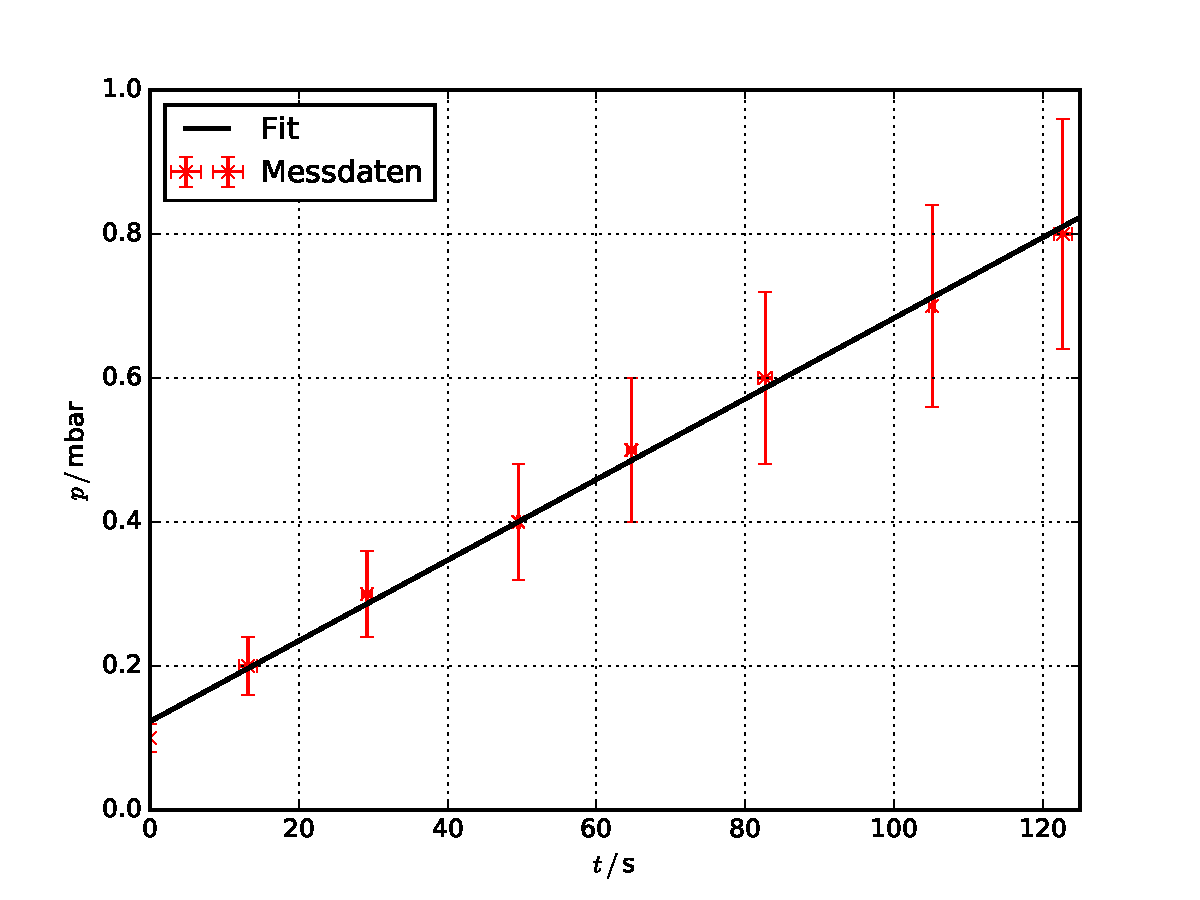
\includegraphics[width=1\textwidth]{plots/LeckrateDreh0_1.pdf}
        \caption{Darstellung der Messwerte aus Tabelle \ref{tab:leck_Dreh1} mit gefitteter Ausgleichsgerade.}
        \label{fig:Leck_Dreh1}
    \end{subfigure}
    \begin{subfigure}{0.45\textwidth}
        \centering
        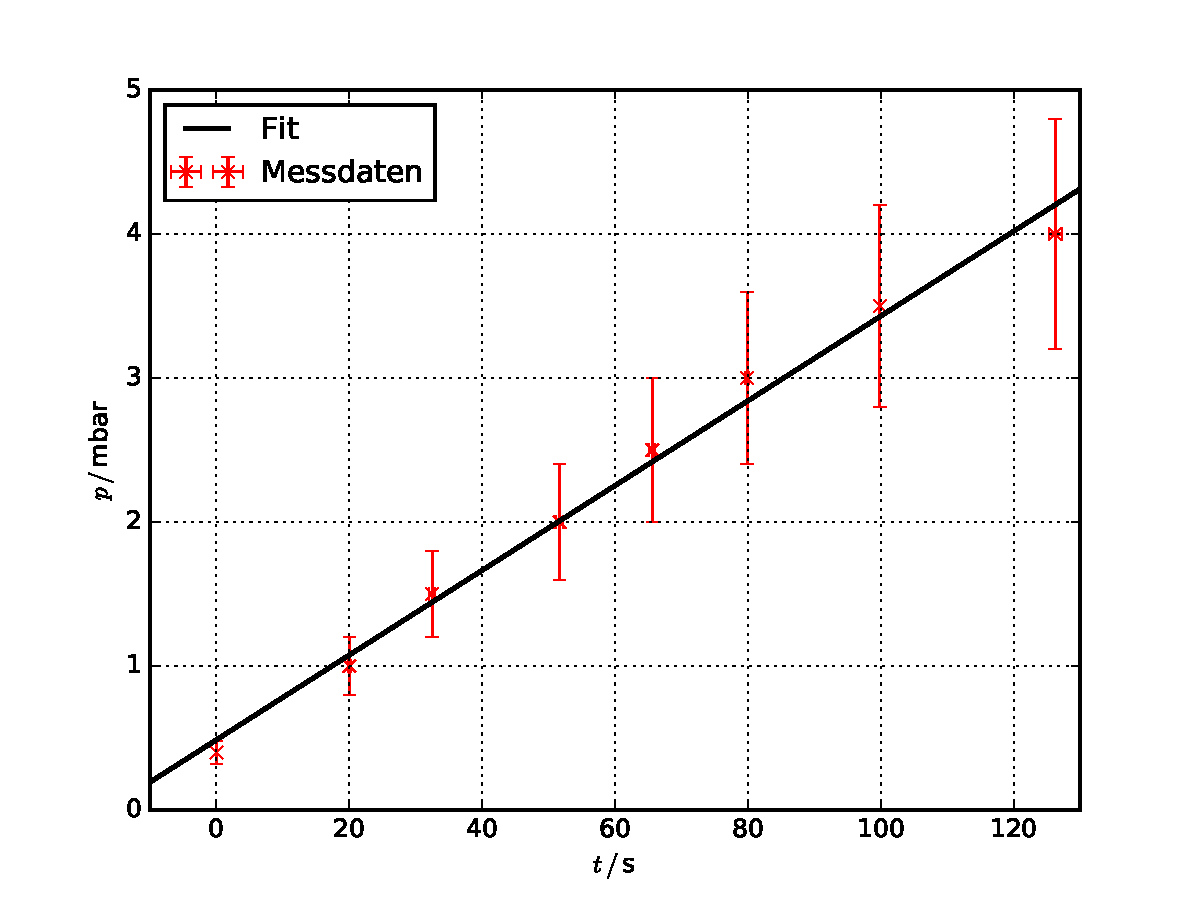
\includegraphics[width=1\textwidth]{plots/LeckrateDreh0_4.pdf}
        \caption{Darstellung der Messwerte aus Tabelle \ref{tab:leck_Dreh2} mit gefitteter Ausgleichsgerade.}
        \label{fig:Leck_Dreh2}
    \end{subfigure}
    \caption{Darstellung der Leckratenmessung bei der Drehschieberpumpe bei den Gleichgewichtsdrücken $p_\symup{g}=0,1$\, mbar und $p_\symup{g}=0,4$\, mbar.}
      \label{fig:leck_dreh_groß1}
\end{figure}
\begin{figure}
    \centering
    \begin{subfigure}{0.45\textwidth}
        \centering
        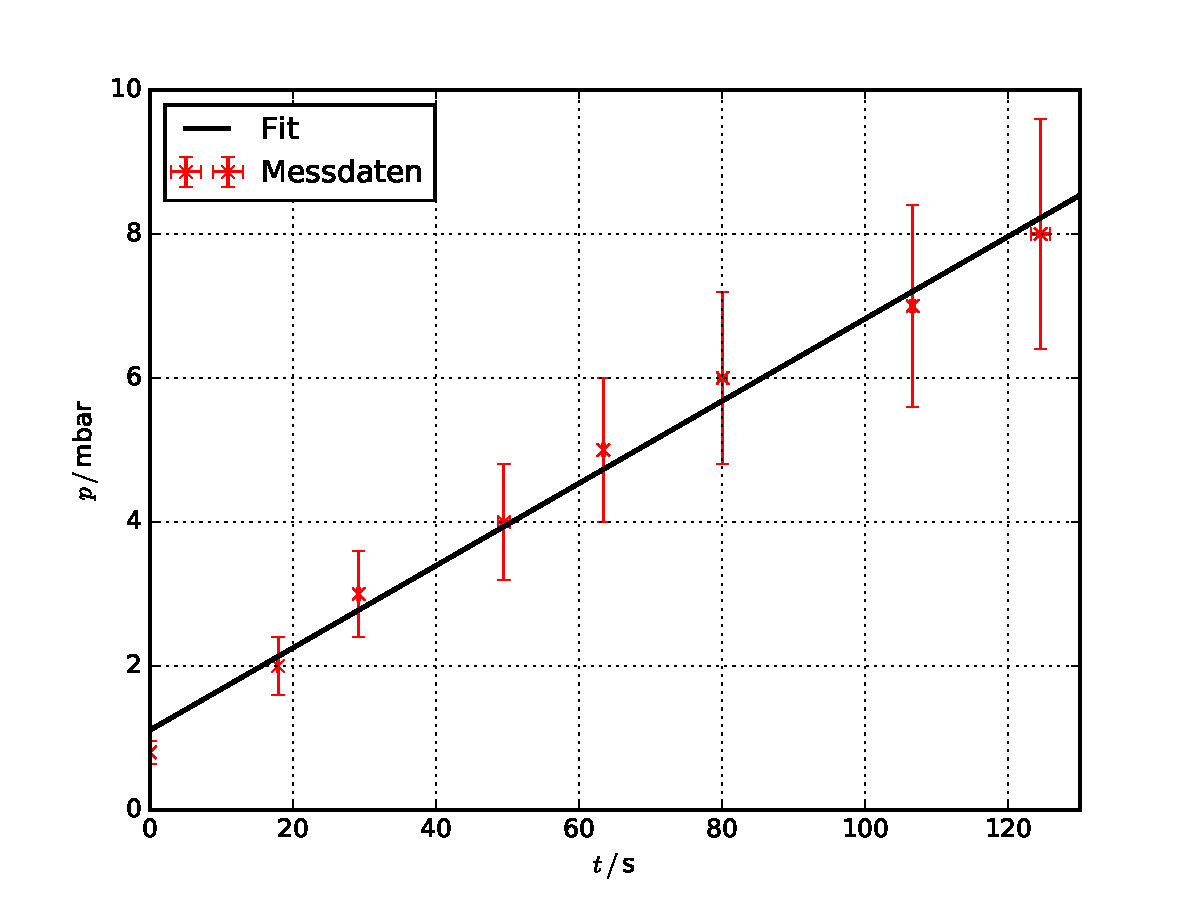
\includegraphics[width=1\textwidth]{plots/LeckrateDreh0_8.pdf}
        \caption{Darstellung der Messwerte aus Tabelle \ref{tab:leck_Dreh3} mit gefitteter Ausgleichsgerade.}
        \label{fig:Leck_Dreh3}
    \end{subfigure}
    \begin{subfigure}{0.45\textwidth}
        \centering
        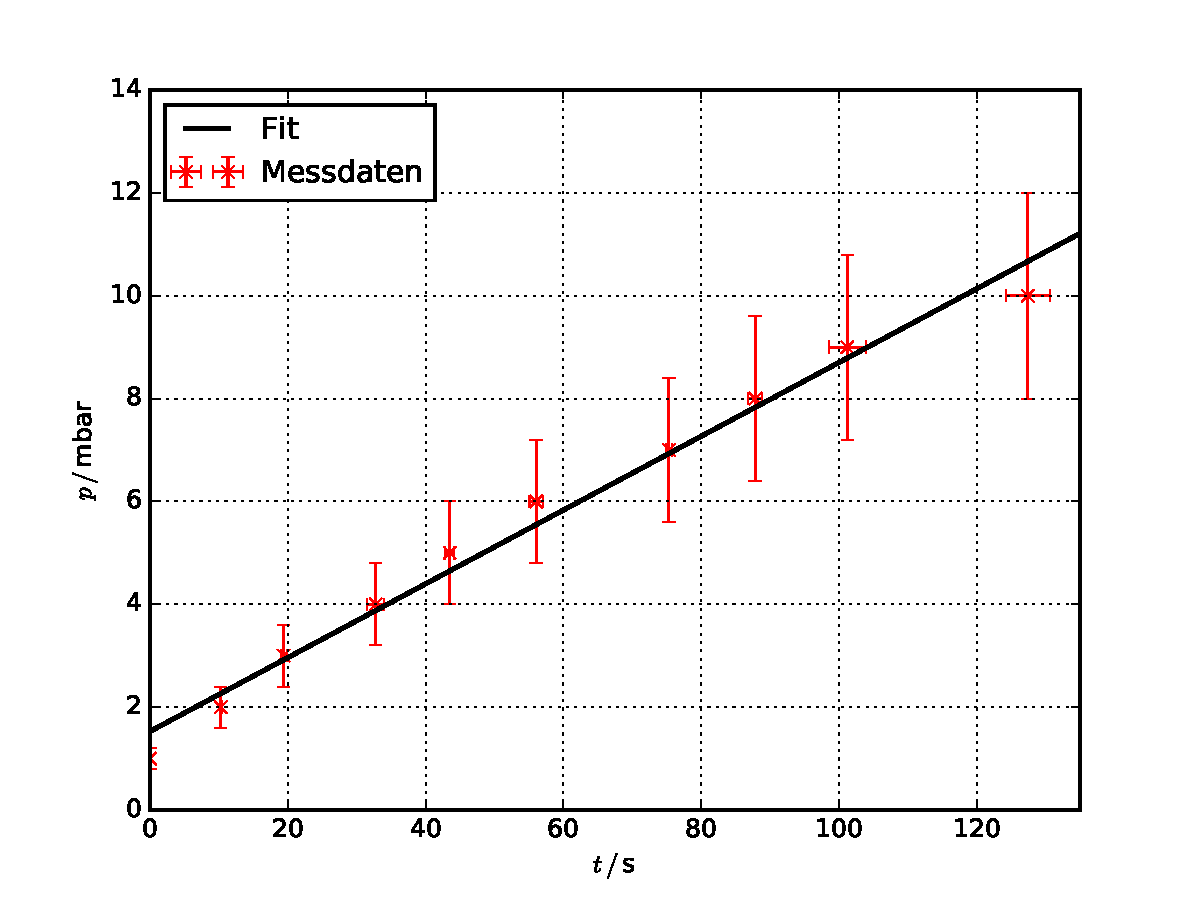
\includegraphics[width=1\textwidth]{plots/LeckrateDreh1.pdf}
        \caption{Darstellung der Messwerte aus Tabelle \ref{tab:leck_Dreh3} mit gefitteter Ausgleichsgerade.}
        \label{fig:Leck_Dreh3}
    \end{subfigure}
    \caption{Darstellung Leckratenmessung bei der Drehschieberpumpe bei den Gleichgewichtsdrücken $p_\symup{g}=0,8$\, mbar und $p_\symup{g}=1$\, mbar.}
      \label{fig:leck_dreh_groß2}
\end{figure}
Für die Parameter der Ausgleichsgeraden ergeben sich die in \ref{eq:regression_dreh_druck_1}, \ref{eq:regression_dreh_druck_2}, \ref{eq:regression_dreh_druck_3}
und \ref{eq:regression_dreh_druck_4} aufgetragenen Werte. Desweiteren sind dort die berechneten Saugleistungen. Diese
werden nach Gleichung \ref{eq:SQ} mit den Steigungen der Ausgleichsgeraden $a$ durch $S=\frac{S}{V}\cdot a$ bestimmt.
Das Volumen bei dieser Messung beträgt $V=(11,0 \pm 0,8)$\,l.

\begin{align}
  \label{eq:regression_dreh_druck_1}
  \begin{aligned}
  \text{Gleichgewichtsdruck} \quad p_\symup{g}&=0,1\,\symup{mbar} \\
  m&= (0,0056 \pm 0,0001)\, \frac{\symup{mbar}}{\symup{s}}\\
  b&= (0,123 \pm 0,009)\,\symup{mbar}\\
  S_1&=(0,6 \pm 0,1)\,\frac{\symup{l}}{\symup{s}}
\end{aligned}
\end{align}
\begin{align}
  \label{eq:regression_dreh_druck_2}
  \begin{aligned}
  \text{Gleichgewichtsdruck}\quad p_\symup{g}&=0,4\,\symup{mbar}\\
  m&= (0,029 \pm 0,001)\, \frac{\symup{mbar}}{\symup{s}}\\
  b&= (0,049 \pm 0,08)\,\symup{mbar}\\
  S_2&=(0,8 \pm 0,2)\,\frac{\symup{l}}{\symup{s}}
\end{aligned}
\end{align}
\begin{align}
  \label{eq:regression_dreh_druck_3}
  \begin{aligned}
  \text{Gleichgewichtsdruck}\quad p_\symup{g}&=0,8\,\symup{mbar}\\
  m&= (0,057 \pm 0,002)\, \frac{\symup{mbar}}{\symup{s}}\\
  b&= (1,1 \pm 0,2)\,\symup{mbar}\\
  S_3&=(0,8 \pm 0,2)\,\frac{\symup{l}}{\symup{s}}
\end{aligned}
\end{align}
\begin{align}
  \label{eq:regression_dreh_druck_4}
  \begin{aligned}
  \text{Gleichgewichtsdruck}\quad p_\symup{g}&=1\,\symup{mbar}\\
  m&= ( 0,072 \pm 0,003)\, \frac{\symup{mbar}}{\symup{s}}\\
  b&= (1,5 \pm 0,2)\,\symup{mbar}\\
  S_4&=(0,8 \pm 0,2)\,\frac{\symup{l}}{\symup{s}}
\end{aligned}
\end{align}
Abschließend wird das Saugvermögen der Drehschieberpumpe gegen den Druck aus den einzelnen Messungen aufgetragen. Hierbei
stehen die horizontalen Balken in Abbildung \ref{fig:SaugDreh} für den Druckbereich für den diese Saugleistung bestimmt wurde
und die vertikalen Balken geben den Fehler an. Die Bezeichnungen sind wie folgt gewählt: $S_{\text{theo}}$ steht für die
Angabe des Herstellers, da dort keine Angaben zum Fehler gemacht werden, konnte dieser nicht eingetragen werden \cite{Anleitung}.
Die aus dem Exponentialfit bestimmte gemittelte Saugleistung ist mit $S_\symup{g}$ benannt. $S_\symup{lin_i}$ zeigen die Werte
aus den logarithmirten Fits und $S_\symup{leck_i}$ sind die Werte aus den Leckratenmessungen.
\begin{figure}[H]
  \centering
  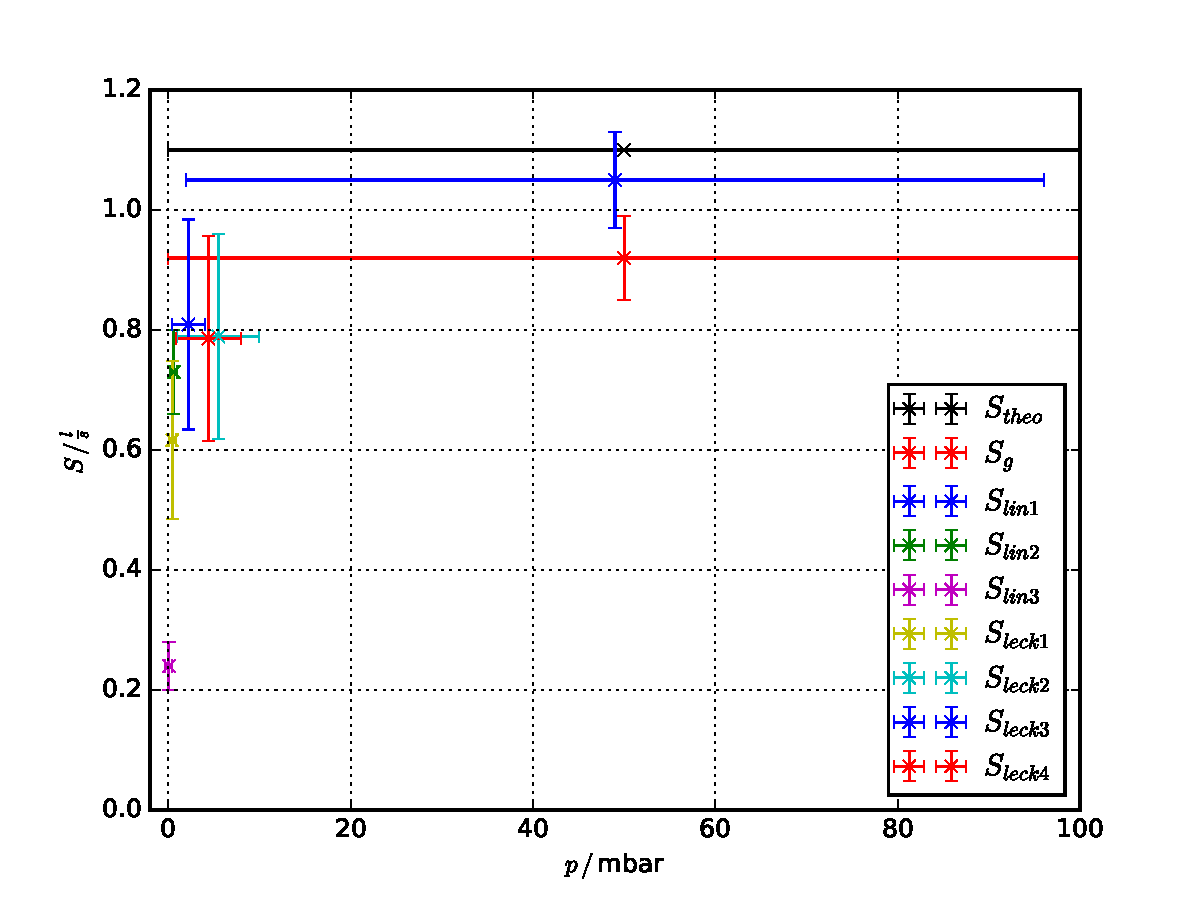
\includegraphics[width=0.7\textwidth]{plots/SaugverDreh.pdf}
  \caption{Darstellung der bestimmten Saugvermögen und die theoretische Angabe des Herstellers.}
  \label{fig:SaugDreh}
\end{figure}
\subsection{Turbomolekularpumpe}
\subsubsection{Evakuierungsmessung}
Die in \ref{tab:EvakuierungskurveTurbo} aufgetragenen Drücke $p$ haben durch die Messungenauigkeit des Glühkathoden-Vakuummeters
einen Fehler von $\pm \, 10$\%.

\begin{table}[H]
\centering
\caption{Messwerte zur Bestimmung der Evakuierungskurve der Turbomolekularpumpe.}
\label{tab:EvakuierungskurveTurbo}
\begin{tabular}{c|c|c|c|c|c|c|c}
  \toprule
$p$/\,mbar & $ln\left(\frac{p(t)-p_\symup{E}}{p_0-p_\symup{E}}\right)$ & $t_1$/\,s & $t_2$/\,s & $t_3$/\,s & $t_4$/\,s & $t_5$/\,s & $t_\symup{m}$/\,s\\
\midrule
$2\cdot 10^{-2}$ \pm \,$2\cdot 10^{-3}$&-1,36 \pm \, 0,14 & 0,99& 1,18& 1,05& 0,99& 0,92& 1,03 \pm \, 0,04\\
$4\cdot 10^{-4}$ \pm \,$2\cdot 10^{-5}$&-2,97 \pm \, 0,14 & 2,42& 2,70& 2,55& 2,51& 2,52& 2,54 \pm \, 0,05\\
$2\cdot 10^{-4}$ \pm \,$2\cdot 10^{-5}$&-3,67 \pm \, 0,14 & 2,83& 3,33& 3,11& 3,25& 3,15& 3,13 \pm \, 0,09\\
$6\cdot 10^{-5}$ \pm \,$6\cdot 10^{-6}$&-4,88 \pm \, 0,14 & 4,70& 4,93& 4,94& 4,84& 4,83& 4,85 \pm \, 0,04\\
$4\cdot 10^{-5}$ \pm \,$4\cdot 10^{-6}$&-5,30 \pm \, 0,14 & 5,23& 5,55& 5,44& 5,49& 5,35& 5,41 \pm \, 0,06\\
$2\cdot 10^{-5}$ \pm \,$2\cdot 10^{-6}$&-6,02 \pm \, 0,15 & 6,62& 6,97& 6,85& 6,91& 6,59& 6,79 \pm \, 0,08 \\
\bottomrule
\end{tabular}
\end{table}
Die in Tabelle \ref{tab:EvakuierungskurveTurbo} aufgetragenen Messwerte für den Druck sind in Abbildung \ref{fig:EvaTurboExp} in
dargestellt.
\begin{figure}[H]
  \centering
  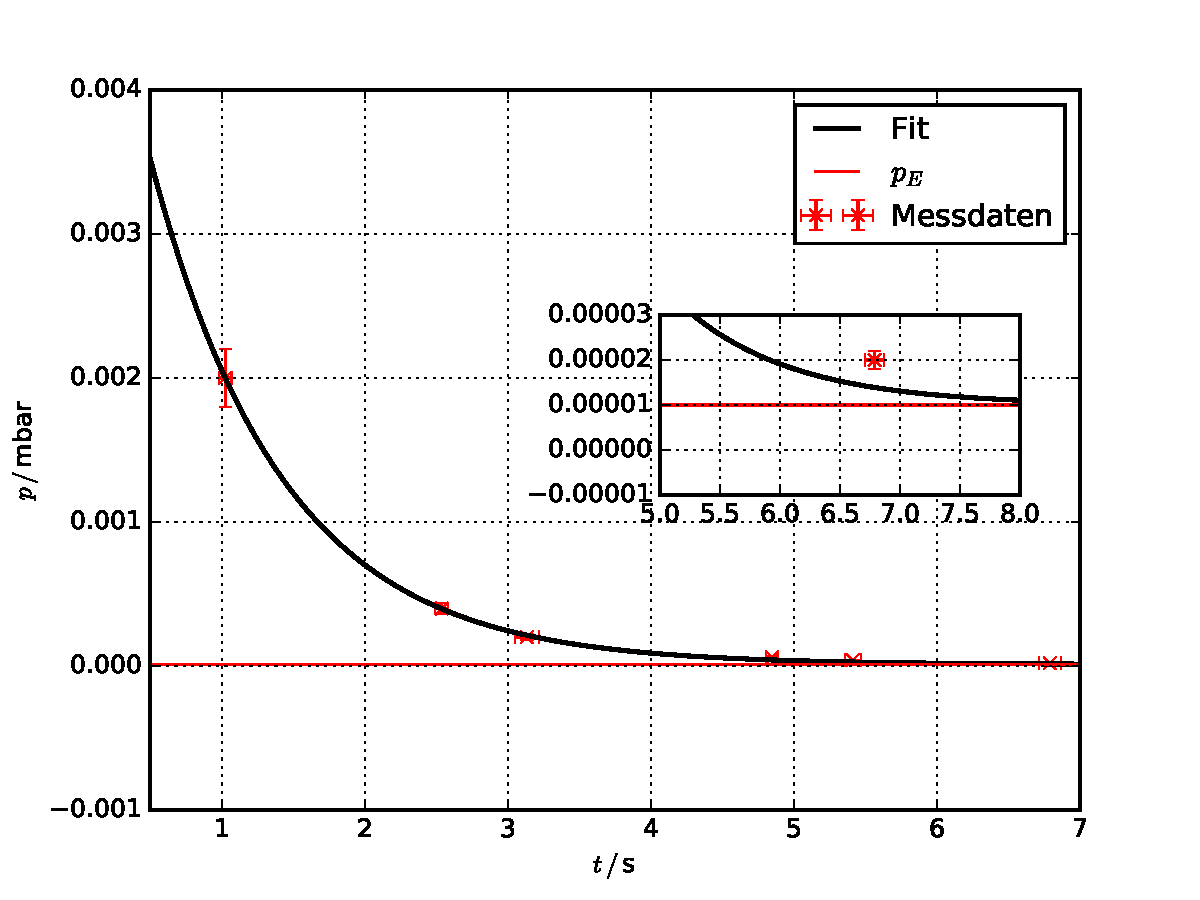
\includegraphics[width=0.7\textwidth]{plots/EvakuierungTurboExp.pdf}
  \caption{Plot der in Tabelle \ref{tab:EvakuierungskurveTurbo} aufgelisteten Messwerte mit exponentiellem Fit. Zusätzlich ist eine Vergrößerung
  des Bereichs 7\,s$\leq t\leq$10\,s dargestellt.}
  \label{fig:EvaTurboExp}
\end{figure}
Der in Abbildung \ref{fig:EvaTurboExp} verwendetet Fit folgt der Gleichung \ref{eq:Drehexpfit}
wobei für den Parameter $c$ der Enddruck $p_\symup{E}=(1\cdot 10^{-6} \pm 5 \cdot 10^{-7})$\,mbar angegeben ist.
Die anderen Parameter wurden zu
\begin{align}
  a&= (0,0060 \pm 0,0001)\,\,\symup{mbar}\\
  b&= (1,08 \pm 0,02)\,\frac{1}{\symup{s}}
\end{align}
Aus dem Parameter $b$ lässt sich nun ein gemitteltes Saugvermögen $S_\symup{g}$ berechnen.
Aus Gleichung \ref{eq:pt} folgt $b=\frac{S}{V}$. Mit einem Volumen von $V=(11,0 \pm 0,8)$\,l und ergibt sich:
\begin{equation}
  S_\symup{g}= b \cdot V =(1,08 \pm 0,02)\,\frac{1}{\symup{s}} \cdot (11,0 \pm 0,8)\,\symup{l} =(11,9 \pm 0,9)\,\frac{\symup{l}}{\symup{s}}
  \label{eq:Saugvermögen}
\end{equation}
Um das Saugvermögen in Abhängigkeit des Drucks zu bestimmen wurden
in Abbildung \ref{fig:EvaTurboLin} die logarithmierten Werte gegen die Zeit aufgetragen.
\begin{figure}[H]
  \centering
  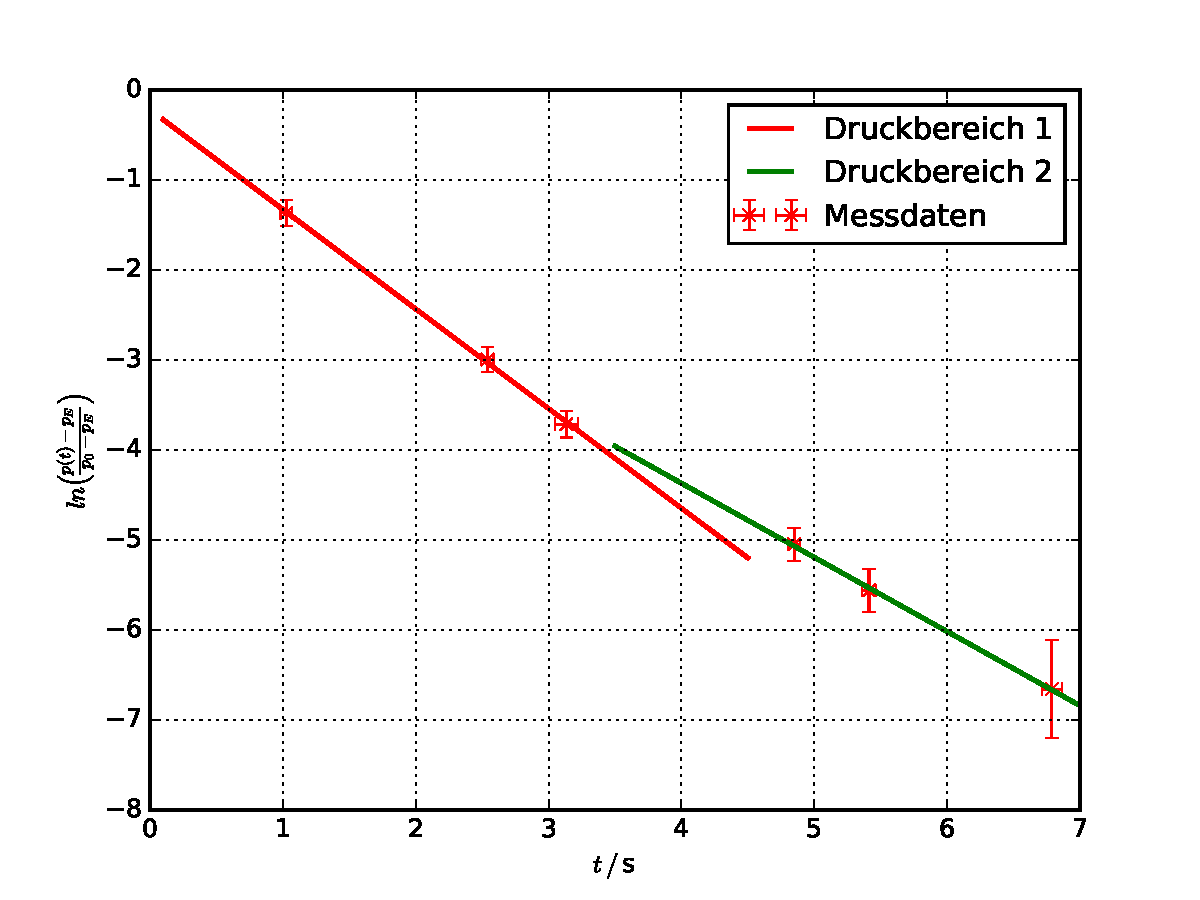
\includegraphics[width=0.7\textwidth]{plots/EvakuierungTurbolin.pdf}
  \caption{Plot der in Tabelle \ref{tab:EvakuierungskurveTurbo} aufgelisteten Messwerte mit linearen Fits der einzelnen Teilbereichen.}
  \label{fig:EvaTurboLin}
\end{figure}
Wie in der Abbildung \ref{fig:EvaDrehLin} zu erkennen, gibt es zwei lineare Bereiche. %,
Diese werden mit Gleichung \ref{eq:Geradengleichung} gefittet.
Mit Hilfe von Regressionsberechnungen werden die Parameter der einzelnen Geraden bestimmt.
Um das Saugvermögen $S=-a\cdot V$ zu bestimmen wird jetzt die Steigung $a$ verwendet:
\begin{align}
  \label{eq: regression_turbo_druck_1}
  \begin{aligned}
  \text{Druckbereich 1} \quad  &  0,0002\,\symup{mbar}\leq p \leq  0,002\,\symup{mbar} \\
  m&= (-1,11 \pm 0,03) \frac{1}{\symup{s}}\\
  b&= -0,21 \pm 0,07\\
  S_1&= (12,2 \pm 0,9)\,\frac{\symup{l}}{\symup{s}}
\end{aligned}
\end{align}
\begin{align}
  \label{eq: regression_turbo_druck_2}
  \begin{aligned}
  \text{Druckbereich 2} \quad  & 2 \cdot 10^{-5}\,\symup{mbar}\leq p \leq 6 \cdot 10^{-5}\,\symup{mbar} \\
  m&=  (-0,82 \pm 0,02)\frac{1}{\symup{s}}\\
  b&= -1,1 \pm 0,1\\
  S_2&= (9,1 \pm 0,7)\,\frac{\symup{l}}{\symup{s}}
\end{aligned}
\end{align}
\subsubsection{Leckratenmessung}
Die Aufgenommenen Messwerte für die vier unterschiedlichen Gleichgewichtsdrücke sind in den Tabellen
\ref{tab:leck_turbo1},\ref{tab:leck_turbo2}, \ref{tab:leck_turbo3} und \ref{tab:leck_turbo4} aufgelistet.
\begin{table}[H]
\centering
\caption{Messwerte der Leckratenmessung der Turbomolekularpumpe mit Gleichgewichtsdruck $p_\symup{g}=1 \cdot 10^{-4}$\, mbar.}
\label{tab:leck_turbo1}
\begin{tabular}{c|c|c|c|c}
  \toprule
$p$/\,mbar & $t_1$/\,s & $t_2$/\,s & $t_3$/\,s & $t_\symup{m}$/\,s\\
\midrule
$(4 \pm 0,4)\cdot 10^{-4}$& 1,64 &   1,7&  1,32& $(1,6 \pm 0,1 )$ \\
$(6 \pm 0,6)\cdot 10^{-4}$& 2,74 &  2,83&  2,46& $( 2,7 \pm 0,1)$\\
$(8 \pm 0,8)\cdot 10^{-4}$& 3,89 &  3,76&  3,48& $(3,7 \pm 0,1 )$ \\
$(2 \pm 0,2)\cdot 10^{-3}$& 9,85 &  9,72&  9,32& $(9,6 \pm 0,2 )$\\
$(4 \pm 0,4)\cdot 10^{-3}$& 18,40& 18,13& 17,66& $(18,1 \pm 0,2)$  \\
$(6 \pm 0,6)\cdot 10^{-3}$& 25,21& 25,21& 24,86& $(25,1 \pm 0,1)$ \\
$(8 \pm 0,8)\cdot 10^{-3}$& 32,16& 31,96& 31,68& $(32,0 \pm 0,1)$ \\
\bottomrule
\end{tabular}
\end{table}
\begin{table}[H]
\centering
\caption{Messwerte der Leckratenmessung der Turbomolekularpumpe mit Gleichgewichtsdruck $p_\symup{g}=2 \cdot 10^{-4}$\, mbar,}
\label{tab:leck_turbo2}
\begin{tabular}{c|c|c|c|c|c|c}
  \toprule
$p$/\,mbar & $t_1$/\,s & $t_2$/\,s & $t_3$/\,s & $t_4$/\,s & $t_5$/\,s & $t_\symup{m}$/\,s\\
\midrule
$(6 \pm 0,6)\cdot 10^{-4}$& 0,92  &1,05 & 1,07 &1,06 & 1,05& $(1,03 \pm 0,03)$  \\
$(8 \pm 0,8)\cdot 10^{-4}$& 1,55  &1,77 & 1,51 &1,75 & 1,48& $(1,61\pm 0,06)$  \\
$(2 \pm 0,2)\cdot 10^{-3}$& 4,43  &5,83 & 4,26 &5,80 & 4,45& $(5,0\pm 0,4)$   \\
$(4 \pm 0,4)\cdot 10^{-3}$& 8,81  &11,08& 8,50 &10,97& 8,56& $(9,6\pm 0,6)$  \\
$(6 \pm 0,6)\cdot 10^{-3}$& 12,52 &15,83& 12,19&15,59& 12,26& $(13,7\pm 0,8)$\\
$(8 \pm 0,8)\cdot 10^{-3}$& 15,96 &20,19& 15,45&19,76& 15,2& $(17\pm 1)$ \\
\bottomrule
\end{tabular}
\end{table}
\begin{table}[H]
\centering
\caption{Messwerte der Leckratenmessung der Turbomolekularpumpe mit Gleichgewichtsdruck $p_\symup{g}=3 \cdot 10^{-5}$\, mbar.}
\label{tab:leck_turbo3}
\begin{tabular}{c|c|c|c|c|c}
  \toprule
$p$/\,mbar & $t_1$/\,s & $t_2$/\,s & $t_3$/\,s & $t_4$/\,s & $t_\symup{m}$/\,s\\
\midrule
$(8 \pm 0,8)\cdot 10^{-4}$&  1,77&  0,6 &   0,7&  0,98& $(1,0 \pm 0,3)$\\
$(2 \pm 0,2)\cdot 10^{-4}$&  5,26&  4,0 &  3,48&  4,58& $(4,3 \pm 0,4)$ \\
$(4 \pm 0,4)\cdot 10^{-4}$& 11,68&  9,6 &  8,23& 10,73& $(10,1 \pm 0,7)$  \\
$(6 \pm 0,6)\cdot 10^{-4}$& 17,56& 14,78& 12,79& 17,01& $(15,5 \pm 1)$ \\
$(8 \pm 0,8)\cdot 10^{-4}$& 22,93& 20,24& 17,01& 23,12& $(20,8 \pm 1)$\\
$(2 \pm 0,2)\cdot 10^{-3}$& 58,08&  60,2& 41,35& 68,07& $(56,9 \pm 6)$ \\
\bottomrule
\end{tabular}
\end{table}
\begin{table}[H]
\centering
\caption{Messwerte der Leckratenmessung der Turbomolekularpumpe mit Gleichgewichtsdruck $p_\symup{g}=8 \cdot 10^{-5}$\, mbar.}
\label{tab:leck_turbo4}
\begin{tabular}{c|c|c|c|c}
  \toprule
$p$/\,mbar & $t_1$/\,s & $t_2$/\,s & $t_3$/\,s & $t_\symup{m}$/\,s\\
\midrule
$(4 \pm 0,4)\cdot 10^{-4}$& 2,29 &2,69   &2,40 &$(2,5 \pm 0,1) $\\
$(6 \pm 0,6)\cdot 10^{-4}$& 3,89 &4,35   &4,34 &$(4,2 \pm 0,2)  $\\
$(8 \pm 0,8)\cdot 10^{-4}$& 5,28 &5,74   &6,35 &$(5,8 \pm 0,3) $\\
$(2 \pm 0,2)\cdot 10^{-3}$& 13,07& 13,95 &18,15&$(15 \pm 2) $\\
$(4 \pm 0,4)\cdot 10^{-3}$& 24,26& 25,19 &35,31&$(28 \pm 4) $\\
$(6 \pm 0,6)\cdot 10^{-3}$& 33,88& 35,25 &49,92&$(39 \pm 5) $\\
$(8 \pm 0,8)\cdot 10^{-3}$& 42,54& 44,08 &60,02&$(48 \pm 6)$\\
\bottomrule
\end{tabular}
\end{table}
In den Graphiken \ref{fig:leck_turbo_groß1} und \ref{fig:leck_turbo_groß2} sind die Messwerte der vier Leckratenmessungen graphisch aufgetragen.
Es wurden mittels linearer Regression Ausgleichsgeraden der Form \ref{eq:Geradengleichung} bestimmt.
\begin{figure}
    \centering
    \begin{subfigure}{0.45\textwidth}
        \centering
        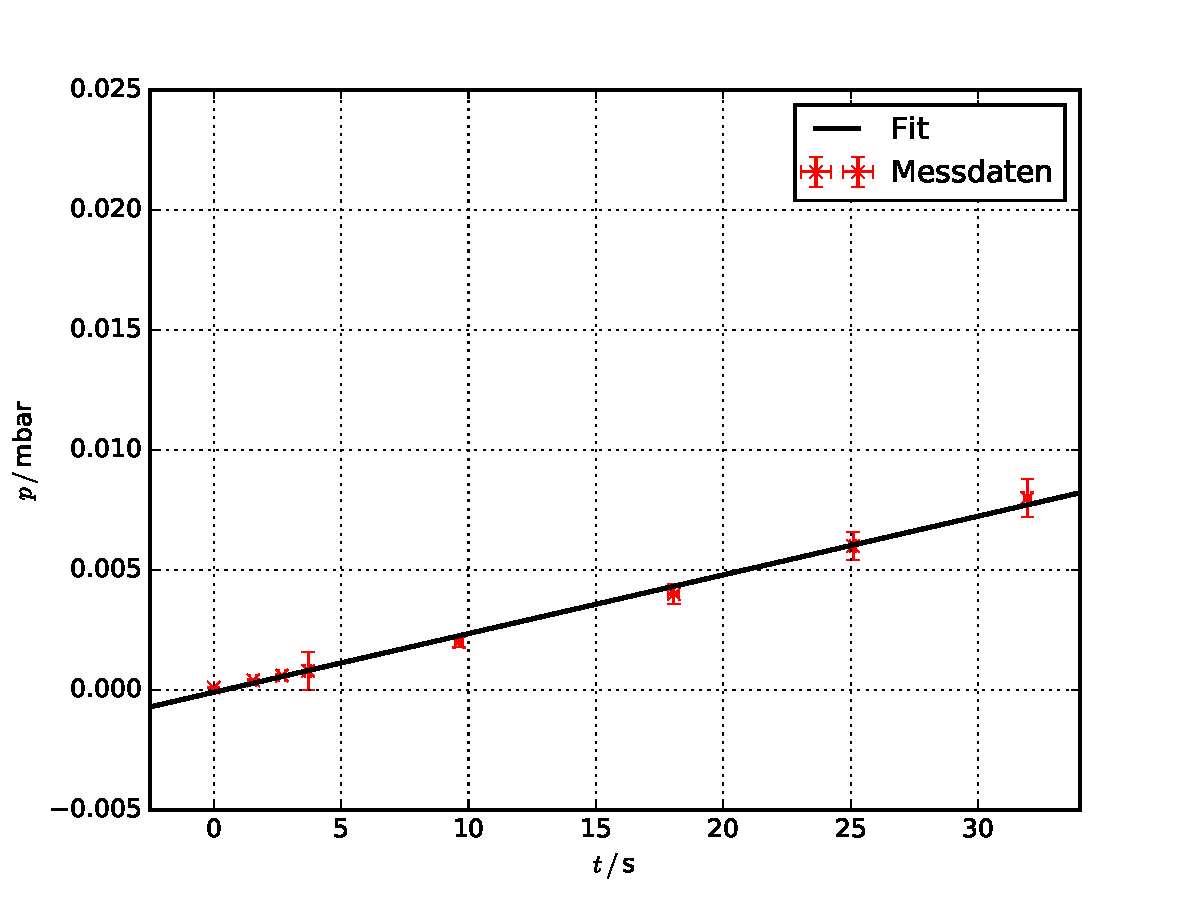
\includegraphics[width=1\textwidth]{plots/LeckrateTurbo1_4.pdf}
        \caption{Darstellung der Messwerte aus Tabelle \ref{tab:leck_turbo1} mit gefitteter Ausgleichsgerade.}
        \label{fig:Leck_turbo1}
    \end{subfigure}
    \begin{subfigure}{0.45\textwidth}
        \centering
        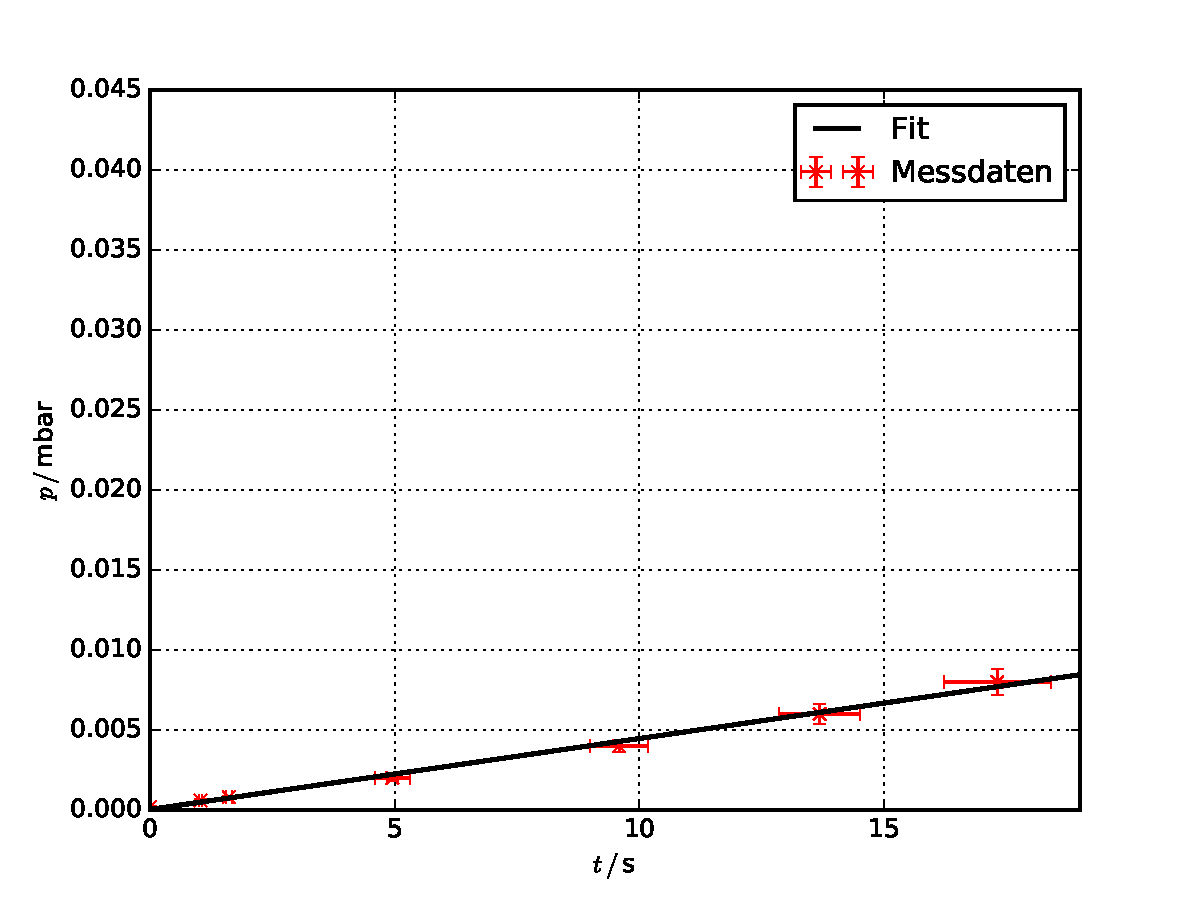
\includegraphics[width=1\textwidth]{plots/LeckrateTurbo2_4.pdf}
        \caption{Darstellung der Messwerte aus Tabelle \ref{tab:leck_turbo2} mit gefitteter Ausgleichsgerade.}
        \label{fig:Leck_turbo2}
    \end{subfigure}
    \caption{Leckratenmessung bei der Turbomolekularpumpe bei den Gleichgewichtsdrücken $p_\symup{g}=1 \cdot 10^{-4}$\, mbar und $p_\symup{g}=2 \cdot 10^{-4}$\, mbar.}
      \label{fig:leck_turbo_groß1}
\end{figure}
\begin{figure}
    \centering
    \begin{subfigure}{0.45\textwidth}
        \centering
        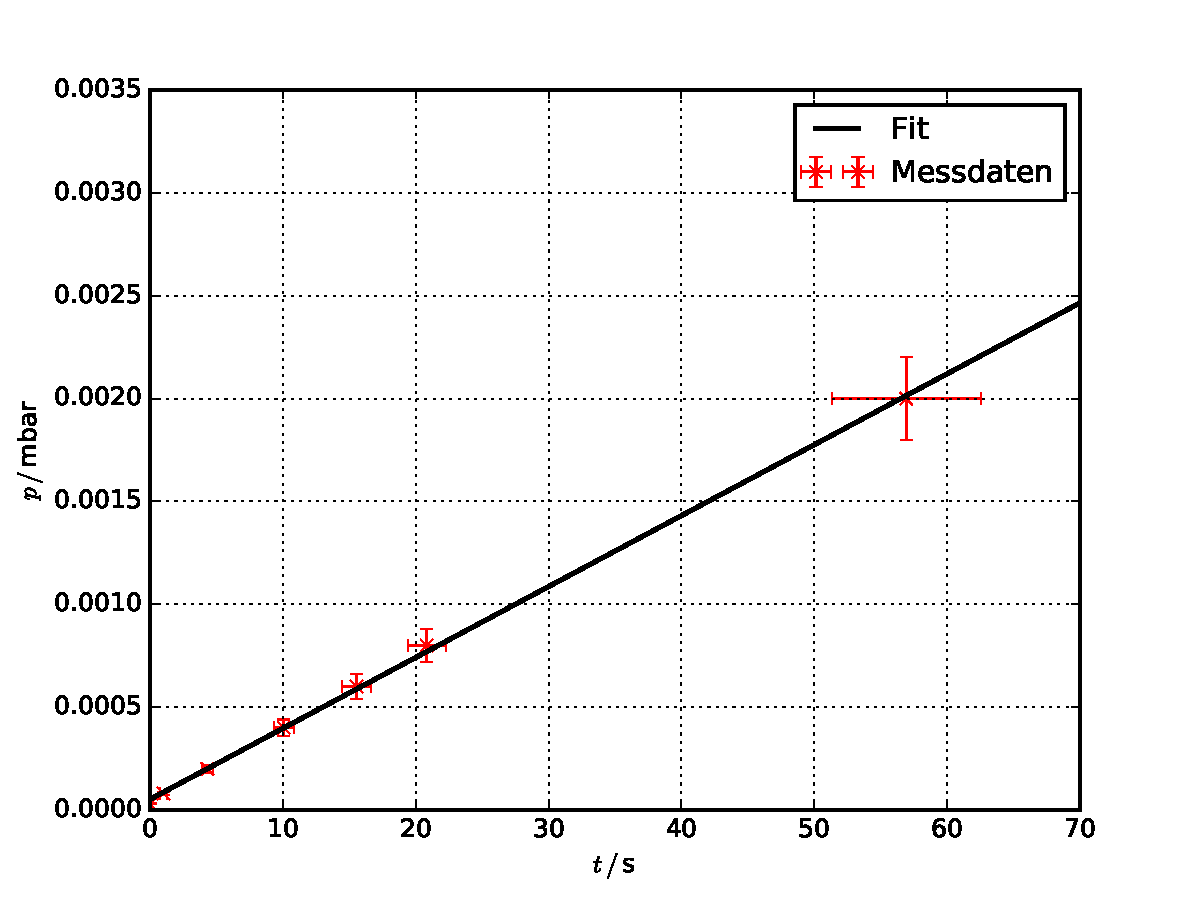
\includegraphics[width=1\textwidth]{plots/LeckrateTurbo3_5.pdf}
        \caption{Darstellung der Messwerte aus Tabelle \ref{tab:leck_turbo3} mit gefitteter Ausgleichsgerade.}
        \label{fig:Leck_turbo3}
    \end{subfigure}
    \begin{subfigure}{0.45\textwidth}
        \centering
        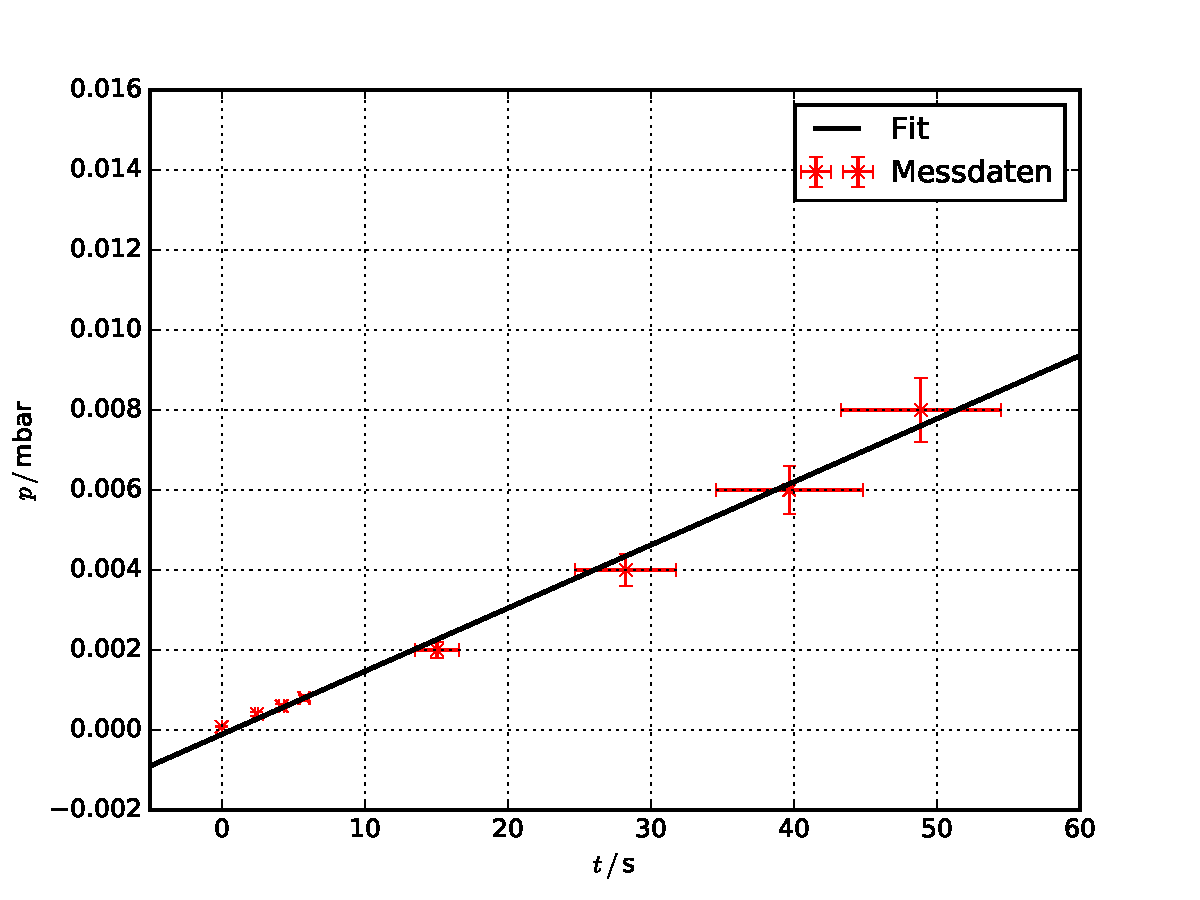
\includegraphics[width=1\textwidth]{plots/LeckrateTurbo8_5.pdf}
        \caption{Darstellung der Messwerte aus Tabelle \ref{tab:leck_turbo3} mit gefitteter Ausgleichsgerade.}
        \label{fig:Leck_turbo3}
    \end{subfigure}
    \caption{Leckratenmessung bei der Turbomolekularpumpe bei den Gleichgewichtsdrücken $p_\symup{g}=3 \cdot 10^{-5}$\, mbar und $p_\symup{g}=8 \cdot 10^{-5}$\, mbar.}
      \label{fig:leck_turbo_groß2}
\end{figure}
Für die Parameter der Ausgleichsgeraden ergeben sich die in \ref{eq:regression_Turbo_druck_1}, \ref{eq:regression_Turbo_druck_2}, \ref{eq:regression_Turbo_druck_3}
und \ref{eq:regression_Turbo_druck_4} aufgetragenen Werte. Desweiteren sind dort die berechneten Saugleistungen. Diese
werden analog zu der Saugvermögensberechnung bei der Drehschieberpumpe bestimmt.
Das Volumen bei dieser Messung beträgt $V=(10,0 \pm 0,8)$\,l.
\begin{align}
  \label{eq:regression_Turbo_druck_1}
  \begin{aligned}
  \text{Gleichgewichtsdruck} \quad p_\symup{g}&=1 \cdot 10^{-4}\,\symup{mbar}\\
  m&= (0,000245 \pm 7\cdot10^{-6})\, \frac{\symup{mbar}}{\symup{s}}\\
  b&= (-0,00009 \pm 0,0001)\,\symup{mbar}\\
  S_1&=(25\pm3)\,\frac{\symup{l}}{\symup{s}}
\end{aligned}
\end{align}
\begin{align}
  \label{eq:regression_Turbo_druck_2}
  \begin{aligned}
  \text{Gleichgewichtsdruck}\quad p_\symup{g}&=2 \cdot 10^{-4}\,\symup{mbar}\\
  m&= (0.00044 \pm 1\cdot10^{-5})\, \frac{\symup{mbar}}{\symup{s}}\\
  b&= (-0,00004 \pm 0,0001)\,\symup{mbar}\\
  S_2&=(22\pm3)\,\frac{\symup{l}}{\symup{s}}
\end{aligned}
\end{align}
\begin{align}
  \label{eq:regression_Turbo_druck_3}
  \begin{aligned}
  \text{Gleichgewichtsdruck}\quad p_\symup{g}&=3 \cdot 10^{-5}\,\symup{mbar}\\
  m&= ( 3,45\cdot10^{-5} \pm 4\cdot10^{-7})\, \frac{\symup{mbar}}{\symup{s}}\\
  b&= (5,2\cdot10^{-5} \pm 9\cdot10^{-6})\,\symup{mbar}\\
  S_3&=(12\pm2)\,\frac{\symup{l}}{\symup{s}}
\end{aligned}
\end{align}
\begin{align}
  \label{eq:regression_Turbo_druck_4}
  \begin{aligned}
  \text{Gleichgewichtsdruck}\quad p_\symup{g}&=8 \cdot 10^{-5}\,\symup{mbar}\\
  m&= (0,000178 \pm 5\cdot10^{-6})\, \frac{\symup{mbar}}{\symup{s}}\\
  b&= (-0,0001 \pm 0,0001)\,\symup{mbar}\\
  S_4&=(20\pm3)\,\frac{\symup{l}}{\symup{s}}
\end{aligned}
\end{align}
Abschließend wird das Saugvermögen der Turbomolekularpumpe gegen den Druck aus den einzelnen Messungen aufgetragen. Hierbei
stehen die horizontalen Balken in Abbildung \ref{fig:SaugTurbo} für den Druckbereich für den diese Saugleistung bestimmt wurde
und die vertikalen Balken geben den Fehler an. Die Bezeichnungen sind analog zu denen in \ref{fig:SaugDreh}.
\begin{figure}[H]
  \centering
  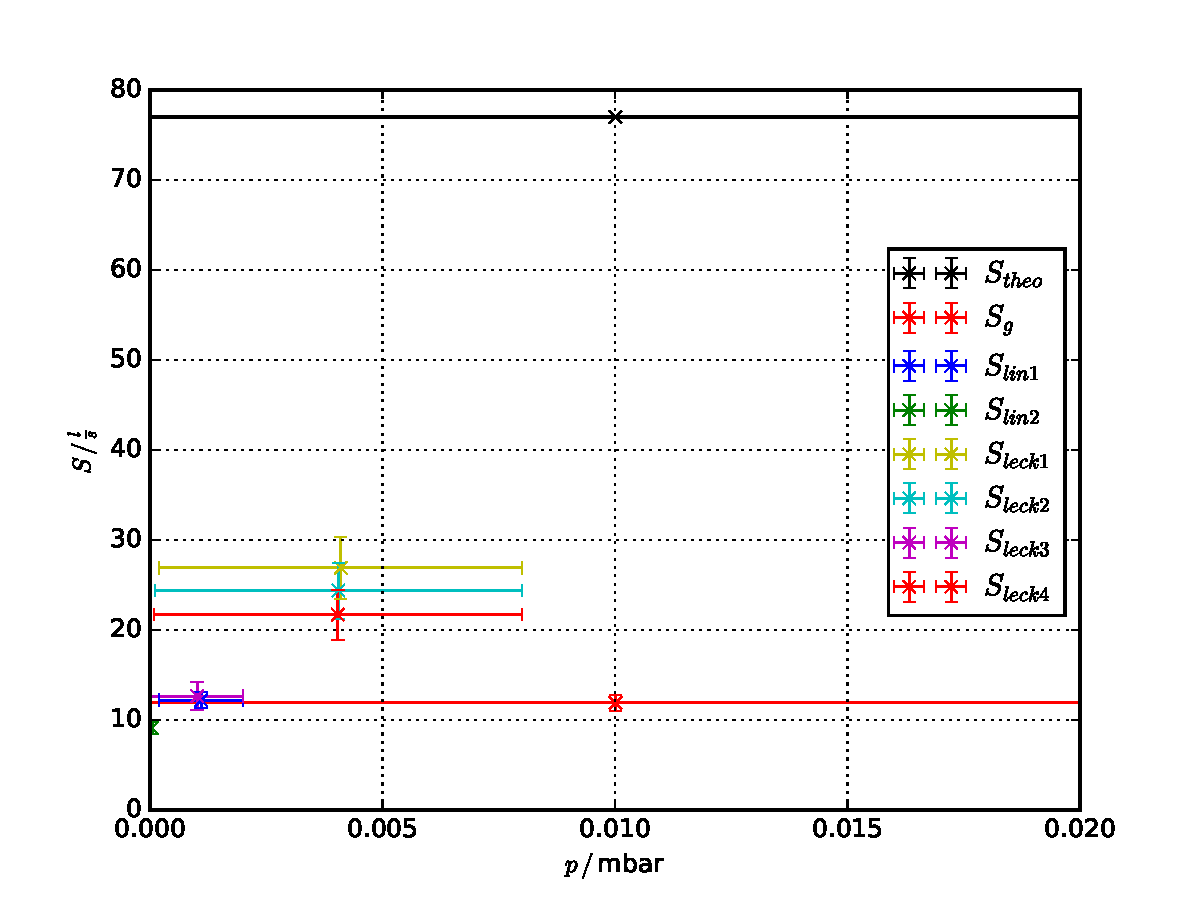
\includegraphics[width=0.7\textwidth]{plots/SaugverTurbo.pdf}
  \caption{Darstellung der bestimmten Saugvermögen und die theoretische Angabe des Herstellers für die Turbomolekularpumpe.}
  \label{fig:SaugTurbo}
\end{figure}
